\documentclass{article}

\usepackage{tikz}

\author{Soren Soroush}
\title{TikZ Learning}
\date{\today \\ \small (last edit)}


\begin{document}
\maketitle
% \tableofcontents
% ---------------

\section*{Basic Shapes}

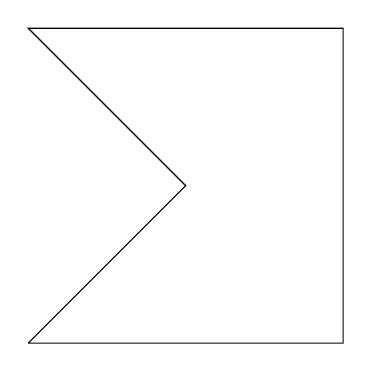
\begin{tikzpicture}
    \draw[] (0,0) -- (4,0) -- (4,4) -- (0,4) -- (2,2) -- (0,0); 
\end{tikzpicture}

\begin{tikzpicture}
    \draw[] (0,0) -- (2,2) -- (2,0) -- cycle; 
    \draw[] (0,0) rectangle (5,5); 
    \draw[] (2,2) parabola (5,5); 
\end{tikzpicture}

\begin{tikzpicture}
    \draw[] (0,0) rectangle (5,3);
    \draw[] (0,0) parabola (5,3); 
\end{tikzpicture}

\begin{tikzpicture}
    \draw[]  (2,0) .. controls (0,0) and (2,0) .. (4,4); 
\end{tikzpicture}

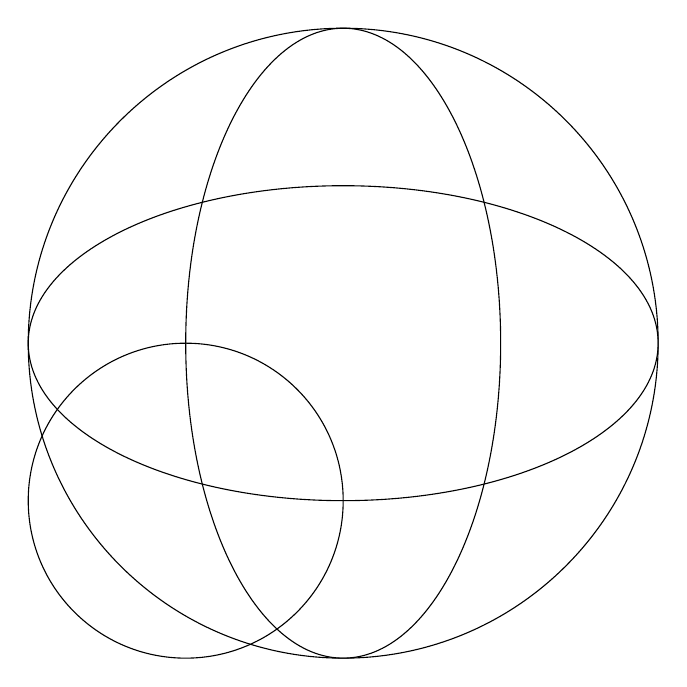
\begin{tikzpicture}
    \draw[] (0,0) circle (2cm);
    \draw[] (2,2) circle (4cm); 
    \draw[] (2,2) ellipse (4cm and 2cm);
    \draw[] (2,2) ellipse (2cm and 4cm);
\end{tikzpicture}

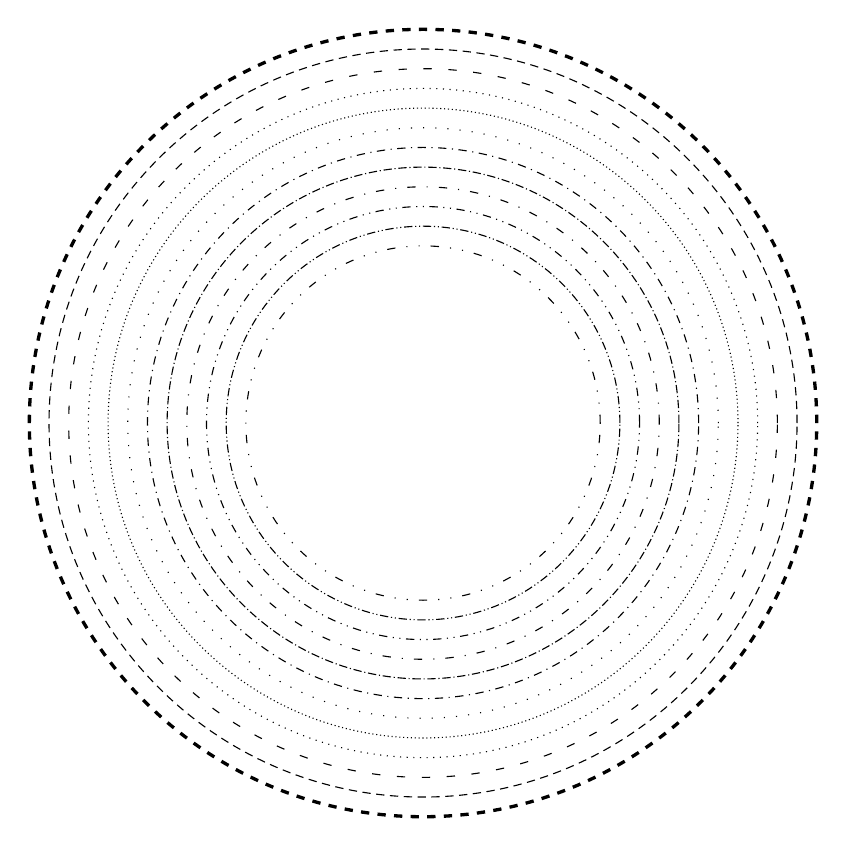
\begin{tikzpicture}
    \draw[dashed, very thick] circle (5cm); 
    \draw[densely dashed] circle (4.75cm); 
    \draw[loosely dashed] circle (4.5cm); 
    \draw[dotted] circle (4.25cm); 
    \draw[densely dotted] circle (4cm); 
    \draw[loosely dotted] circle (3.75cm); 
    \draw[dashdotted] circle (3.5cm); 
    \draw[densely dashdotted] circle (3.25cm); 
    \draw[loosely dashdotted] circle (3cm); 
    \draw[dashdotdotted] circle (2.75cm); 
    \draw[densely dashdotdotted] circle (2.5cm); 
    \draw[loosely dashdotdotted] circle (2.25cm); 
\end{tikzpicture}
% ---------------
\end{document}
